\documentclass[]{article}
\usepackage{lmodern}
\usepackage{amssymb,amsmath}
\usepackage{ifxetex,ifluatex}
\usepackage{fixltx2e} % provides \textsubscript
\ifnum 0\ifxetex 1\fi\ifluatex 1\fi=0 % if pdftex
  \usepackage[T1]{fontenc}
  \usepackage[utf8]{inputenc}
\else % if luatex or xelatex
  \ifxetex
    \usepackage{mathspec}
  \else
    \usepackage{fontspec}
  \fi
  \defaultfontfeatures{Ligatures=TeX,Scale=MatchLowercase}
\fi
% use upquote if available, for straight quotes in verbatim environments
\IfFileExists{upquote.sty}{\usepackage{upquote}}{}
% use microtype if available
\IfFileExists{microtype.sty}{%
\usepackage{microtype}
\UseMicrotypeSet[protrusion]{basicmath} % disable protrusion for tt fonts
}{}
\usepackage[margin=1in]{geometry}
\usepackage{hyperref}
\hypersetup{unicode=true,
            pdftitle={news\_data\_prep},
            pdfborder={0 0 0},
            breaklinks=true}
\urlstyle{same}  % don't use monospace font for urls
\usepackage{color}
\usepackage{fancyvrb}
\newcommand{\VerbBar}{|}
\newcommand{\VERB}{\Verb[commandchars=\\\{\}]}
\DefineVerbatimEnvironment{Highlighting}{Verbatim}{commandchars=\\\{\}}
% Add ',fontsize=\small' for more characters per line
\usepackage{framed}
\definecolor{shadecolor}{RGB}{248,248,248}
\newenvironment{Shaded}{\begin{snugshade}}{\end{snugshade}}
\newcommand{\AlertTok}[1]{\textcolor[rgb]{0.94,0.16,0.16}{#1}}
\newcommand{\AnnotationTok}[1]{\textcolor[rgb]{0.56,0.35,0.01}{\textbf{\textit{#1}}}}
\newcommand{\AttributeTok}[1]{\textcolor[rgb]{0.77,0.63,0.00}{#1}}
\newcommand{\BaseNTok}[1]{\textcolor[rgb]{0.00,0.00,0.81}{#1}}
\newcommand{\BuiltInTok}[1]{#1}
\newcommand{\CharTok}[1]{\textcolor[rgb]{0.31,0.60,0.02}{#1}}
\newcommand{\CommentTok}[1]{\textcolor[rgb]{0.56,0.35,0.01}{\textit{#1}}}
\newcommand{\CommentVarTok}[1]{\textcolor[rgb]{0.56,0.35,0.01}{\textbf{\textit{#1}}}}
\newcommand{\ConstantTok}[1]{\textcolor[rgb]{0.00,0.00,0.00}{#1}}
\newcommand{\ControlFlowTok}[1]{\textcolor[rgb]{0.13,0.29,0.53}{\textbf{#1}}}
\newcommand{\DataTypeTok}[1]{\textcolor[rgb]{0.13,0.29,0.53}{#1}}
\newcommand{\DecValTok}[1]{\textcolor[rgb]{0.00,0.00,0.81}{#1}}
\newcommand{\DocumentationTok}[1]{\textcolor[rgb]{0.56,0.35,0.01}{\textbf{\textit{#1}}}}
\newcommand{\ErrorTok}[1]{\textcolor[rgb]{0.64,0.00,0.00}{\textbf{#1}}}
\newcommand{\ExtensionTok}[1]{#1}
\newcommand{\FloatTok}[1]{\textcolor[rgb]{0.00,0.00,0.81}{#1}}
\newcommand{\FunctionTok}[1]{\textcolor[rgb]{0.00,0.00,0.00}{#1}}
\newcommand{\ImportTok}[1]{#1}
\newcommand{\InformationTok}[1]{\textcolor[rgb]{0.56,0.35,0.01}{\textbf{\textit{#1}}}}
\newcommand{\KeywordTok}[1]{\textcolor[rgb]{0.13,0.29,0.53}{\textbf{#1}}}
\newcommand{\NormalTok}[1]{#1}
\newcommand{\OperatorTok}[1]{\textcolor[rgb]{0.81,0.36,0.00}{\textbf{#1}}}
\newcommand{\OtherTok}[1]{\textcolor[rgb]{0.56,0.35,0.01}{#1}}
\newcommand{\PreprocessorTok}[1]{\textcolor[rgb]{0.56,0.35,0.01}{\textit{#1}}}
\newcommand{\RegionMarkerTok}[1]{#1}
\newcommand{\SpecialCharTok}[1]{\textcolor[rgb]{0.00,0.00,0.00}{#1}}
\newcommand{\SpecialStringTok}[1]{\textcolor[rgb]{0.31,0.60,0.02}{#1}}
\newcommand{\StringTok}[1]{\textcolor[rgb]{0.31,0.60,0.02}{#1}}
\newcommand{\VariableTok}[1]{\textcolor[rgb]{0.00,0.00,0.00}{#1}}
\newcommand{\VerbatimStringTok}[1]{\textcolor[rgb]{0.31,0.60,0.02}{#1}}
\newcommand{\WarningTok}[1]{\textcolor[rgb]{0.56,0.35,0.01}{\textbf{\textit{#1}}}}
\usepackage{graphicx,grffile}
\makeatletter
\def\maxwidth{\ifdim\Gin@nat@width>\linewidth\linewidth\else\Gin@nat@width\fi}
\def\maxheight{\ifdim\Gin@nat@height>\textheight\textheight\else\Gin@nat@height\fi}
\makeatother
% Scale images if necessary, so that they will not overflow the page
% margins by default, and it is still possible to overwrite the defaults
% using explicit options in \includegraphics[width, height, ...]{}
\setkeys{Gin}{width=\maxwidth,height=\maxheight,keepaspectratio}
\IfFileExists{parskip.sty}{%
\usepackage{parskip}
}{% else
\setlength{\parindent}{0pt}
\setlength{\parskip}{6pt plus 2pt minus 1pt}
}
\setlength{\emergencystretch}{3em}  % prevent overfull lines
\providecommand{\tightlist}{%
  \setlength{\itemsep}{0pt}\setlength{\parskip}{0pt}}
\setcounter{secnumdepth}{0}
% Redefines (sub)paragraphs to behave more like sections
\ifx\paragraph\undefined\else
\let\oldparagraph\paragraph
\renewcommand{\paragraph}[1]{\oldparagraph{#1}\mbox{}}
\fi
\ifx\subparagraph\undefined\else
\let\oldsubparagraph\subparagraph
\renewcommand{\subparagraph}[1]{\oldsubparagraph{#1}\mbox{}}
\fi

%%% Use protect on footnotes to avoid problems with footnotes in titles
\let\rmarkdownfootnote\footnote%
\def\footnote{\protect\rmarkdownfootnote}

%%% Change title format to be more compact
\usepackage{titling}

% Create subtitle command for use in maketitle
\providecommand{\subtitle}[1]{
  \posttitle{
    \begin{center}\large#1\end{center}
    }
}

\setlength{\droptitle}{-2em}

  \title{news\_data\_prep}
    \pretitle{\vspace{\droptitle}\centering\huge}
  \posttitle{\par}
    \author{}
    \preauthor{}\postauthor{}
    \date{}
    \predate{}\postdate{}
  

\begin{document}
\maketitle

\begin{Shaded}
\begin{Highlighting}[]
\KeywordTok{library}\NormalTok{(tidyverse)}
\end{Highlighting}
\end{Shaded}

\begin{verbatim}
## -- Attaching packages ------------------------------------------------ tidyverse 1.2.1 --
\end{verbatim}

\begin{verbatim}
## v ggplot2 3.2.0     v purrr   0.3.2
## v tibble  2.1.3     v dplyr   0.8.3
## v tidyr   0.8.3     v stringr 1.4.0
## v readr   1.3.1     v forcats 0.4.0
\end{verbatim}

\begin{verbatim}
## Warning: package 'dplyr' was built under R version 3.6.1
\end{verbatim}

\begin{verbatim}
## -- Conflicts --------------------------------------------------- tidyverse_conflicts() --
## x dplyr::filter() masks stats::filter()
## x dplyr::lag()    masks stats::lag()
\end{verbatim}

\begin{Shaded}
\begin{Highlighting}[]
\KeywordTok{library}\NormalTok{(caret)}
\end{Highlighting}
\end{Shaded}

\begin{verbatim}
## Warning: package 'caret' was built under R version 3.6.1
\end{verbatim}

\begin{verbatim}
## Loading required package: lattice
\end{verbatim}

\begin{verbatim}
## 
## Attaching package: 'caret'
\end{verbatim}

\begin{verbatim}
## The following object is masked from 'package:purrr':
## 
##     lift
\end{verbatim}

\begin{Shaded}
\begin{Highlighting}[]
\KeywordTok{library}\NormalTok{(corrplot)}
\end{Highlighting}
\end{Shaded}

\begin{verbatim}
## Warning: package 'corrplot' was built under R version 3.6.1
\end{verbatim}

\begin{verbatim}
## corrplot 0.84 loaded
\end{verbatim}

\begin{Shaded}
\begin{Highlighting}[]
\KeywordTok{library}\NormalTok{(party)}
\end{Highlighting}
\end{Shaded}

\begin{verbatim}
## Warning: package 'party' was built under R version 3.6.1
\end{verbatim}

\begin{verbatim}
## Loading required package: grid
\end{verbatim}

\begin{verbatim}
## Loading required package: mvtnorm
\end{verbatim}

\begin{verbatim}
## Loading required package: modeltools
\end{verbatim}

\begin{verbatim}
## Loading required package: stats4
\end{verbatim}

\begin{verbatim}
## Loading required package: strucchange
\end{verbatim}

\begin{verbatim}
## Warning: package 'strucchange' was built under R version 3.6.1
\end{verbatim}

\begin{verbatim}
## Loading required package: zoo
\end{verbatim}

\begin{verbatim}
## Warning: package 'zoo' was built under R version 3.6.1
\end{verbatim}

\begin{verbatim}
## 
## Attaching package: 'zoo'
\end{verbatim}

\begin{verbatim}
## The following objects are masked from 'package:base':
## 
##     as.Date, as.Date.numeric
\end{verbatim}

\begin{verbatim}
## Loading required package: sandwich
\end{verbatim}

\begin{verbatim}
## Warning: package 'sandwich' was built under R version 3.6.1
\end{verbatim}

\begin{verbatim}
## 
## Attaching package: 'strucchange'
\end{verbatim}

\begin{verbatim}
## The following object is masked from 'package:stringr':
## 
##     boundary
\end{verbatim}

\begin{Shaded}
\begin{Highlighting}[]
\KeywordTok{library}\NormalTok{(gbm)}
\end{Highlighting}
\end{Shaded}

\begin{verbatim}
## Warning: package 'gbm' was built under R version 3.6.1
\end{verbatim}

\begin{verbatim}
## Loaded gbm 2.1.5
\end{verbatim}

\begin{Shaded}
\begin{Highlighting}[]
\KeywordTok{library}\NormalTok{(reshape2)}
\end{Highlighting}
\end{Shaded}

\begin{verbatim}
## 
## Attaching package: 'reshape2'
\end{verbatim}

\begin{verbatim}
## The following object is masked from 'package:tidyr':
## 
##     smiths
\end{verbatim}

\begin{Shaded}
\begin{Highlighting}[]
\KeywordTok{library}\NormalTok{(caTools)}
\end{Highlighting}
\end{Shaded}

\begin{verbatim}
## Warning: package 'caTools' was built under R version 3.6.1
\end{verbatim}

\begin{Shaded}
\begin{Highlighting}[]
\KeywordTok{set.seed}\NormalTok{(}\DecValTok{1234}\NormalTok{)}
\end{Highlighting}
\end{Shaded}

\hypertarget{read-datasets}{%
\section{0. Read datasets}\label{read-datasets}}

\begin{Shaded}
\begin{Highlighting}[]
\NormalTok{news_data <-}\StringTok{ }\KeywordTok{read.csv}\NormalTok{(}\StringTok{'Data/dat_train.csv'}\NormalTok{)}

\KeywordTok{str}\NormalTok{(news_data)}
\end{Highlighting}
\end{Shaded}

\begin{verbatim}
## 'data.frame':    20000 obs. of  61 variables:
##  $ url                          : Factor w/ 20000 levels "http://mashable.com/2013/01/07/amazon-instant-video-browser/",..: 1 2 3 4 5 6 7 8 9 10 ...
##  $ timedelta                    : int  731 731 731 731 731 731 731 731 731 731 ...
##  $ n_tokens_title               : int  12 9 9 9 13 10 8 12 11 10 ...
##  $ n_tokens_content             : int  219 255 211 531 1072 370 960 989 97 231 ...
##  $ n_unique_tokens              : num  0.664 0.605 0.575 0.504 0.416 ...
##  $ n_non_stop_words             : num  1 1 1 1 1 ...
##  $ n_non_stop_unique_tokens     : num  0.815 0.792 0.664 0.666 0.541 ...
##  $ num_hrefs                    : int  4 3 3 9 19 2 21 20 2 4 ...
##  $ num_self_hrefs               : int  2 1 1 0 19 2 20 20 0 1 ...
##  $ num_imgs                     : int  1 1 1 1 20 0 20 20 0 1 ...
##  $ num_videos                   : int  0 0 0 0 0 0 0 0 0 1 ...
##  $ average_token_length         : num  4.68 4.91 4.39 4.4 4.68 ...
##  $ num_keywords                 : int  5 4 6 7 7 9 10 9 7 5 ...
##  $ data_channel_is_lifestyle    : int  0 0 0 0 0 0 1 0 0 0 ...
##  $ data_channel_is_entertainment: int  1 0 0 1 0 0 0 0 0 0 ...
##  $ data_channel_is_bus          : int  0 1 1 0 0 0 0 0 0 0 ...
##  $ data_channel_is_socmed       : int  0 0 0 0 0 0 0 0 0 0 ...
##  $ data_channel_is_tech         : int  0 0 0 0 1 1 0 1 1 0 ...
##  $ data_channel_is_world        : int  0 0 0 0 0 0 0 0 0 1 ...
##  $ kw_min_min                   : int  0 0 0 0 0 0 0 0 0 0 ...
##  $ kw_max_min                   : num  0 0 0 0 0 0 0 0 0 0 ...
##  $ kw_avg_min                   : num  0 0 0 0 0 0 0 0 0 0 ...
##  $ kw_min_max                   : int  0 0 0 0 0 0 0 0 0 0 ...
##  $ kw_max_max                   : int  0 0 0 0 0 0 0 0 0 0 ...
##  $ kw_avg_max                   : num  0 0 0 0 0 0 0 0 0 0 ...
##  $ kw_min_avg                   : num  0 0 0 0 0 0 0 0 0 0 ...
##  $ kw_max_avg                   : num  0 0 0 0 0 0 0 0 0 0 ...
##  $ kw_avg_avg                   : num  0 0 0 0 0 0 0 0 0 0 ...
##  $ self_reference_min_shares    : num  496 0 918 0 545 8500 545 545 0 0 ...
##  $ self_reference_max_shares    : num  496 0 918 0 16000 8500 16000 16000 0 0 ...
##  $ self_reference_avg_sharess   : num  496 0 918 0 3151 ...
##  $ weekday_is_monday            : int  1 1 1 1 1 1 1 1 1 1 ...
##  $ weekday_is_tuesday           : int  0 0 0 0 0 0 0 0 0 0 ...
##  $ weekday_is_wednesday         : int  0 0 0 0 0 0 0 0 0 0 ...
##  $ weekday_is_thursday          : int  0 0 0 0 0 0 0 0 0 0 ...
##  $ weekday_is_friday            : int  0 0 0 0 0 0 0 0 0 0 ...
##  $ weekday_is_saturday          : int  0 0 0 0 0 0 0 0 0 0 ...
##  $ weekday_is_sunday            : int  0 0 0 0 0 0 0 0 0 0 ...
##  $ is_weekend                   : int  0 0 0 0 0 0 0 0 0 0 ...
##  $ LDA_00                       : num  0.5003 0.7998 0.2178 0.0286 0.0286 ...
##  $ LDA_01                       : num  0.3783 0.05 0.0333 0.4193 0.0288 ...
##  $ LDA_02                       : num  0.04 0.0501 0.0334 0.4947 0.0286 ...
##  $ LDA_03                       : num  0.0413 0.0501 0.0333 0.0289 0.0286 ...
##  $ LDA_04                       : num  0.0401 0.05 0.6822 0.0286 0.8854 ...
##  $ global_subjectivity          : num  0.522 0.341 0.702 0.43 0.514 ...
##  $ global_sentiment_polarity    : num  0.0926 0.1489 0.3233 0.1007 0.281 ...
##  $ global_rate_positive_words   : num  0.0457 0.0431 0.0569 0.0414 0.0746 ...
##  $ global_rate_negative_words   : num  0.0137 0.01569 0.00948 0.02072 0.01213 ...
##  $ rate_positive_words          : num  0.769 0.733 0.857 0.667 0.86 ...
##  $ rate_negative_words          : num  0.231 0.267 0.143 0.333 0.14 ...
##  $ avg_positive_polarity        : num  0.379 0.287 0.496 0.386 0.411 ...
##  $ min_positive_polarity        : num  0.1 0.0333 0.1 0.1364 0.0333 ...
##  $ max_positive_polarity        : num  0.7 0.7 1 0.8 1 0.6 1 1 0.8 0.5 ...
##  $ avg_negative_polarity        : num  -0.35 -0.119 -0.467 -0.37 -0.22 ...
##  $ min_negative_polarity        : num  -0.6 -0.125 -0.8 -0.6 -0.5 -0.4 -0.5 -0.5 -0.125 -0.5 ...
##  $ max_negative_polarity        : num  -0.2 -0.1 -0.133 -0.167 -0.05 ...
##  $ title_subjectivity           : num  0.5 0 0 0 0.455 ...
##  $ title_sentiment_polarity     : num  -0.188 0 0 0 0.136 ...
##  $ abs_title_subjectivity       : num  0 0.5 0.5 0.5 0.0455 ...
##  $ abs_title_sentiment_polarity : num  0.188 0 0 0 0.136 ...
##  $ shares                       : int  593 711 1500 1200 505 855 556 891 3600 710 ...
\end{verbatim}

\begin{Shaded}
\begin{Highlighting}[]
\CommentTok{#unique(news_data$n_non_stop_words)}



\CommentTok{#pairs(news_data)}
\end{Highlighting}
\end{Shaded}

\#1. Visualisation plots

\begin{Shaded}
\begin{Highlighting}[]
\NormalTok{num<-}\KeywordTok{unlist}\NormalTok{(}\KeywordTok{lapply}\NormalTok{(news_data, is.numeric))}
\NormalTok{news_data_cor<-news_data[,num]}
\NormalTok{cor.matrix<-}\KeywordTok{cor}\NormalTok{(news_data_cor)}
\KeywordTok{corrplot}\NormalTok{(cor.matrix, }\DataTypeTok{order=}\StringTok{"hclust"}\NormalTok{, }\DataTypeTok{tl.pos=}\StringTok{'n'}\NormalTok{)}
\end{Highlighting}
\end{Shaded}

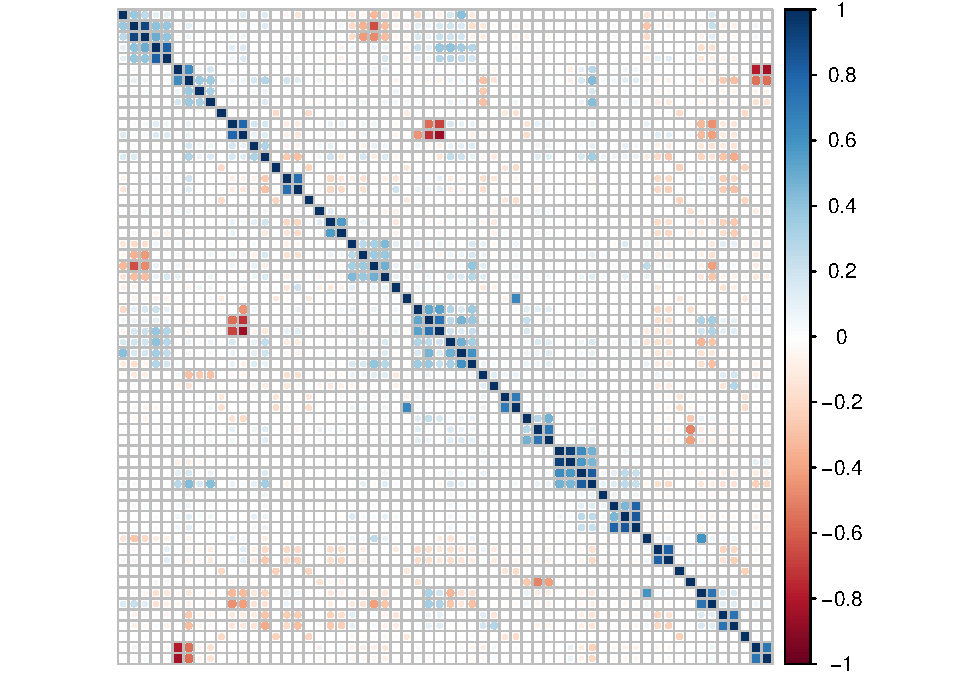
\includegraphics{news_data_prep_files/figure-latex/unnamed-chunk-3-1.pdf}

\begin{Shaded}
\begin{Highlighting}[]
\NormalTok{highcor<-}\KeywordTok{findCorrelation}\NormalTok{(cor.matrix, }\DataTypeTok{cutoff=}\FloatTok{0.9}\NormalTok{, }\DataTypeTok{exact=}\OtherTok{TRUE}\NormalTok{, }\DataTypeTok{name=}\OtherTok{TRUE}\NormalTok{)}

 
\CommentTok{#distribution of target variable }
\KeywordTok{table}\NormalTok{(news_data}\OperatorTok{$}\NormalTok{popular)}
\end{Highlighting}
\end{Shaded}

\begin{verbatim}
## < table of extent 0 >
\end{verbatim}

\hypertarget{data-enginering}{%
\section{Data enginering}\label{data-enginering}}

\begin{Shaded}
\begin{Highlighting}[]
\NormalTok{news_data}\OperatorTok{$}\NormalTok{weekday_is_monday <-}\StringTok{ }\KeywordTok{as.factor}\NormalTok{(news_data}\OperatorTok{$}\NormalTok{weekday_is_monday )}
\NormalTok{news_data}\OperatorTok{$}\NormalTok{weekday_is_tuesday <-}\StringTok{ }\KeywordTok{as.factor}\NormalTok{(news_data}\OperatorTok{$}\NormalTok{weekday_is_tuesday )}
\NormalTok{news_data}\OperatorTok{$}\NormalTok{weekday_is_wednesday <-}\StringTok{ }\KeywordTok{as.factor}\NormalTok{(news_data}\OperatorTok{$}\NormalTok{weekday_is_wednesday )}
\NormalTok{news_data}\OperatorTok{$}\NormalTok{weekday_is_thursday <-}\StringTok{ }\KeywordTok{as.factor}\NormalTok{(news_data}\OperatorTok{$}\NormalTok{weekday_is_thursday )}
\NormalTok{news_data}\OperatorTok{$}\NormalTok{weekday_is_friday <-}\StringTok{ }\KeywordTok{as.factor}\NormalTok{(news_data}\OperatorTok{$}\NormalTok{weekday_is_friday )}
\NormalTok{news_data}\OperatorTok{$}\NormalTok{weekday_is_saturday <-}\StringTok{ }\KeywordTok{as.factor}\NormalTok{(news_data}\OperatorTok{$}\NormalTok{weekday_is_saturday )}
\NormalTok{news_data}\OperatorTok{$}\NormalTok{weekday_is_sunday <-}\StringTok{ }\KeywordTok{as.factor}\NormalTok{(news_data}\OperatorTok{$}\NormalTok{weekday_is_sunday )}
\NormalTok{news_data}\OperatorTok{$}\NormalTok{is_weekend <-}\StringTok{ }\KeywordTok{as.factor}\NormalTok{(news_data}\OperatorTok{$}\NormalTok{is_weekend )}

\NormalTok{news_data}\OperatorTok{$}\NormalTok{popular<-}\KeywordTok{as.factor}\NormalTok{(}\KeywordTok{ifelse}\NormalTok{(news_data}\OperatorTok{$}\NormalTok{shares}\OperatorTok{>}\DecValTok{1400}\NormalTok{,}\StringTok{"yes"}\NormalTok{,}\StringTok{"no"}\NormalTok{))}
\end{Highlighting}
\end{Shaded}

\hypertarget{testtrain}{%
\section{Test/Train}\label{testtrain}}

\begin{Shaded}
\begin{Highlighting}[]
\CommentTok{## 80% of the sample size}
\NormalTok{smp_size <-}\StringTok{ }\KeywordTok{floor}\NormalTok{(}\FloatTok{0.80} \OperatorTok{*}\StringTok{ }\KeywordTok{nrow}\NormalTok{(news_data))}


\NormalTok{train_ind <-}\StringTok{ }\KeywordTok{sample}\NormalTok{(}\KeywordTok{seq_len}\NormalTok{(}\KeywordTok{nrow}\NormalTok{(news_data)), }\DataTypeTok{size =}\NormalTok{ smp_size)}

\NormalTok{news_train <-}\StringTok{ }\NormalTok{news_data[train_ind, ]}
\NormalTok{news_test <-}\StringTok{ }\NormalTok{news_data[}\OperatorTok{-}\NormalTok{train_ind, ]}
\end{Highlighting}
\end{Shaded}

\hypertarget{model-creation}{%
\section{Model Creation}\label{model-creation}}

\begin{Shaded}
\begin{Highlighting}[]
\NormalTok{myControl <-}\StringTok{ }\KeywordTok{trainControl}\NormalTok{(}
  \DataTypeTok{method =} \StringTok{"cv"}\NormalTok{,}
  \DataTypeTok{number =} \DecValTok{5}\NormalTok{,}
  \DataTypeTok{verboseIter =} \OtherTok{FALSE}
\NormalTok{)}
\NormalTok{model_gbm <-}\StringTok{ }\KeywordTok{train}\NormalTok{(popular }\OperatorTok{~}\StringTok{ }\NormalTok{kw_avg_avg }\OperatorTok{+}
\StringTok{                      }\NormalTok{self_reference_min_shares}\OperatorTok{+}
\StringTok{                      }\NormalTok{is_weekend}\OperatorTok{+}
\StringTok{                      }\NormalTok{kw_min_avg}\OperatorTok{+}
\StringTok{                      }\NormalTok{kw_max_avg}\OperatorTok{+}
\StringTok{                      }\NormalTok{kw_max_max    }\OperatorTok{+}
\StringTok{                      }\NormalTok{self_reference_avg_sharess    }\OperatorTok{+}
\StringTok{                      }\NormalTok{data_channel_is_socmed    }\OperatorTok{+}
\StringTok{                      }\NormalTok{n_unique_tokens       }\OperatorTok{+}
\StringTok{                      }\NormalTok{kw_avg_max}\OperatorTok{+}
\StringTok{                      }\NormalTok{data_channel_is_entertainment }\OperatorTok{+}
\StringTok{                      }\NormalTok{LDA_}\DecValTok{02}    \OperatorTok{+}
\StringTok{                      }\NormalTok{kw_avg_min    }\OperatorTok{+}
\StringTok{                      }\NormalTok{data_channel_is_tech  }\OperatorTok{+}
\StringTok{                      }\NormalTok{LDA_}\DecValTok{00}        \OperatorTok{+}
\StringTok{                      }\NormalTok{LDA_}\DecValTok{01}        \OperatorTok{+}
\StringTok{                      }\NormalTok{title_sentiment_polarity  }\OperatorTok{+}
\StringTok{                      }\NormalTok{weekday_is_saturday   }\OperatorTok{+}
\StringTok{                      }\NormalTok{LDA_}\DecValTok{03} \OperatorTok{+}
\StringTok{                      }\NormalTok{global_subjectivity,}
                     \DataTypeTok{data =}\NormalTok{ news_train ,}
                     \DataTypeTok{method =} \StringTok{"gbm"}\NormalTok{,}
                     \DataTypeTok{trControl =}\NormalTok{ myControl}
\NormalTok{                   )}
\end{Highlighting}
\end{Shaded}

\begin{verbatim}
## Iter   TrainDeviance   ValidDeviance   StepSize   Improve
##      1        1.3807             nan     0.1000    0.0029
##      2        1.3761             nan     0.1000    0.0023
##      3        1.3722             nan     0.1000    0.0019
##      4        1.3686             nan     0.1000    0.0016
##      5        1.3650             nan     0.1000    0.0016
##      6        1.3619             nan     0.1000    0.0010
##      7        1.3590             nan     0.1000    0.0012
##      8        1.3559             nan     0.1000    0.0014
##      9        1.3534             nan     0.1000    0.0011
##     10        1.3507             nan     0.1000    0.0011
##     20        1.3302             nan     0.1000    0.0008
##     40        1.3036             nan     0.1000    0.0005
##     60        1.2863             nan     0.1000    0.0003
##     80        1.2748             nan     0.1000    0.0002
##    100        1.2673             nan     0.1000    0.0001
##    120        1.2616             nan     0.1000    0.0000
##    140        1.2571             nan     0.1000    0.0000
##    150        1.2550             nan     0.1000   -0.0000
## 
## Iter   TrainDeviance   ValidDeviance   StepSize   Improve
##      1        1.3778             nan     0.1000    0.0041
##      2        1.3707             nan     0.1000    0.0032
##      3        1.3639             nan     0.1000    0.0031
##      4        1.3585             nan     0.1000    0.0025
##      5        1.3534             nan     0.1000    0.0022
##      6        1.3488             nan     0.1000    0.0020
##      7        1.3446             nan     0.1000    0.0021
##      8        1.3401             nan     0.1000    0.0020
##      9        1.3367             nan     0.1000    0.0015
##     10        1.3323             nan     0.1000    0.0019
##     20        1.3037             nan     0.1000    0.0010
##     40        1.2723             nan     0.1000    0.0001
##     60        1.2563             nan     0.1000    0.0003
##     80        1.2446             nan     0.1000    0.0001
##    100        1.2362             nan     0.1000   -0.0000
##    120        1.2297             nan     0.1000   -0.0000
##    140        1.2240             nan     0.1000    0.0001
##    150        1.2216             nan     0.1000   -0.0000
## 
## Iter   TrainDeviance   ValidDeviance   StepSize   Improve
##      1        1.3759             nan     0.1000    0.0047
##      2        1.3676             nan     0.1000    0.0039
##      3        1.3597             nan     0.1000    0.0034
##      4        1.3529             nan     0.1000    0.0031
##      5        1.3468             nan     0.1000    0.0030
##      6        1.3410             nan     0.1000    0.0026
##      7        1.3355             nan     0.1000    0.0023
##      8        1.3305             nan     0.1000    0.0021
##      9        1.3259             nan     0.1000    0.0018
##     10        1.3219             nan     0.1000    0.0016
##     20        1.2896             nan     0.1000    0.0009
##     40        1.2569             nan     0.1000    0.0006
##     60        1.2403             nan     0.1000    0.0003
##     80        1.2292             nan     0.1000    0.0002
##    100        1.2202             nan     0.1000   -0.0002
##    120        1.2136             nan     0.1000   -0.0001
##    140        1.2060             nan     0.1000   -0.0001
##    150        1.2034             nan     0.1000   -0.0001
## 
## Iter   TrainDeviance   ValidDeviance   StepSize   Improve
##      1        1.3806             nan     0.1000    0.0027
##      2        1.3756             nan     0.1000    0.0023
##      3        1.3717             nan     0.1000    0.0019
##      4        1.3682             nan     0.1000    0.0015
##      5        1.3649             nan     0.1000    0.0016
##      6        1.3622             nan     0.1000    0.0012
##      7        1.3593             nan     0.1000    0.0011
##      8        1.3562             nan     0.1000    0.0014
##      9        1.3538             nan     0.1000    0.0011
##     10        1.3517             nan     0.1000    0.0010
##     20        1.3306             nan     0.1000    0.0007
##     40        1.3035             nan     0.1000    0.0004
##     60        1.2867             nan     0.1000    0.0003
##     80        1.2755             nan     0.1000    0.0001
##    100        1.2681             nan     0.1000    0.0001
##    120        1.2623             nan     0.1000    0.0000
##    140        1.2574             nan     0.1000    0.0000
##    150        1.2556             nan     0.1000   -0.0001
## 
## Iter   TrainDeviance   ValidDeviance   StepSize   Improve
##      1        1.3782             nan     0.1000    0.0037
##      2        1.3714             nan     0.1000    0.0033
##      3        1.3649             nan     0.1000    0.0025
##      4        1.3593             nan     0.1000    0.0026
##      5        1.3535             nan     0.1000    0.0024
##      6        1.3490             nan     0.1000    0.0022
##      7        1.3450             nan     0.1000    0.0016
##      8        1.3412             nan     0.1000    0.0020
##      9        1.3372             nan     0.1000    0.0020
##     10        1.3327             nan     0.1000    0.0019
##     20        1.3034             nan     0.1000    0.0008
##     40        1.2734             nan     0.1000    0.0004
##     60        1.2578             nan     0.1000    0.0001
##     80        1.2471             nan     0.1000    0.0000
##    100        1.2392             nan     0.1000   -0.0000
##    120        1.2334             nan     0.1000    0.0000
##    140        1.2287             nan     0.1000    0.0001
##    150        1.2263             nan     0.1000   -0.0000
## 
## Iter   TrainDeviance   ValidDeviance   StepSize   Improve
##      1        1.3757             nan     0.1000    0.0049
##      2        1.3676             nan     0.1000    0.0038
##      3        1.3605             nan     0.1000    0.0033
##      4        1.3535             nan     0.1000    0.0031
##      5        1.3477             nan     0.1000    0.0026
##      6        1.3415             nan     0.1000    0.0029
##      7        1.3353             nan     0.1000    0.0028
##      8        1.3303             nan     0.1000    0.0021
##      9        1.3255             nan     0.1000    0.0020
##     10        1.3213             nan     0.1000    0.0019
##     20        1.2883             nan     0.1000    0.0013
##     40        1.2569             nan     0.1000    0.0005
##     60        1.2416             nan     0.1000    0.0001
##     80        1.2313             nan     0.1000    0.0001
##    100        1.2229             nan     0.1000   -0.0000
##    120        1.2151             nan     0.1000    0.0000
##    140        1.2086             nan     0.1000   -0.0001
##    150        1.2057             nan     0.1000   -0.0003
## 
## Iter   TrainDeviance   ValidDeviance   StepSize   Improve
##      1        1.3809             nan     0.1000    0.0025
##      2        1.3770             nan     0.1000    0.0018
##      3        1.3731             nan     0.1000    0.0018
##      4        1.3688             nan     0.1000    0.0019
##      5        1.3651             nan     0.1000    0.0015
##      6        1.3621             nan     0.1000    0.0014
##      7        1.3589             nan     0.1000    0.0015
##      8        1.3559             nan     0.1000    0.0013
##      9        1.3536             nan     0.1000    0.0012
##     10        1.3511             nan     0.1000    0.0012
##     20        1.3303             nan     0.1000    0.0007
##     40        1.3027             nan     0.1000    0.0004
##     60        1.2857             nan     0.1000    0.0002
##     80        1.2739             nan     0.1000    0.0001
##    100        1.2664             nan     0.1000    0.0000
##    120        1.2605             nan     0.1000    0.0000
##    140        1.2561             nan     0.1000   -0.0000
##    150        1.2543             nan     0.1000   -0.0000
## 
## Iter   TrainDeviance   ValidDeviance   StepSize   Improve
##      1        1.3786             nan     0.1000    0.0037
##      2        1.3719             nan     0.1000    0.0033
##      3        1.3660             nan     0.1000    0.0026
##      4        1.3605             nan     0.1000    0.0023
##      5        1.3552             nan     0.1000    0.0021
##      6        1.3504             nan     0.1000    0.0022
##      7        1.3451             nan     0.1000    0.0024
##      8        1.3410             nan     0.1000    0.0016
##      9        1.3369             nan     0.1000    0.0018
##     10        1.3327             nan     0.1000    0.0018
##     20        1.3030             nan     0.1000    0.0007
##     40        1.2716             nan     0.1000    0.0003
##     60        1.2545             nan     0.1000    0.0002
##     80        1.2444             nan     0.1000   -0.0000
##    100        1.2366             nan     0.1000    0.0000
##    120        1.2307             nan     0.1000   -0.0001
##    140        1.2258             nan     0.1000    0.0001
##    150        1.2234             nan     0.1000    0.0000
## 
## Iter   TrainDeviance   ValidDeviance   StepSize   Improve
##      1        1.3772             nan     0.1000    0.0040
##      2        1.3689             nan     0.1000    0.0037
##      3        1.3616             nan     0.1000    0.0032
##      4        1.3553             nan     0.1000    0.0026
##      5        1.3486             nan     0.1000    0.0028
##      6        1.3420             nan     0.1000    0.0027
##      7        1.3360             nan     0.1000    0.0029
##      8        1.3309             nan     0.1000    0.0022
##      9        1.3255             nan     0.1000    0.0026
##     10        1.3214             nan     0.1000    0.0018
##     20        1.2878             nan     0.1000    0.0010
##     40        1.2562             nan     0.1000    0.0002
##     60        1.2391             nan     0.1000    0.0001
##     80        1.2277             nan     0.1000    0.0000
##    100        1.2197             nan     0.1000   -0.0001
##    120        1.2139             nan     0.1000   -0.0001
##    140        1.2074             nan     0.1000   -0.0002
##    150        1.2040             nan     0.1000    0.0000
## 
## Iter   TrainDeviance   ValidDeviance   StepSize   Improve
##      1        1.3807             nan     0.1000    0.0026
##      2        1.3766             nan     0.1000    0.0018
##      3        1.3723             nan     0.1000    0.0019
##      4        1.3688             nan     0.1000    0.0018
##      5        1.3657             nan     0.1000    0.0012
##      6        1.3626             nan     0.1000    0.0013
##      7        1.3600             nan     0.1000    0.0012
##      8        1.3573             nan     0.1000    0.0010
##      9        1.3539             nan     0.1000    0.0015
##     10        1.3516             nan     0.1000    0.0010
##     20        1.3313             nan     0.1000    0.0009
##     40        1.3035             nan     0.1000    0.0005
##     60        1.2867             nan     0.1000    0.0002
##     80        1.2755             nan     0.1000    0.0002
##    100        1.2679             nan     0.1000    0.0001
##    120        1.2625             nan     0.1000    0.0000
##    140        1.2577             nan     0.1000    0.0000
##    150        1.2558             nan     0.1000    0.0000
## 
## Iter   TrainDeviance   ValidDeviance   StepSize   Improve
##      1        1.3794             nan     0.1000    0.0033
##      2        1.3729             nan     0.1000    0.0032
##      3        1.3668             nan     0.1000    0.0027
##      4        1.3610             nan     0.1000    0.0028
##      5        1.3560             nan     0.1000    0.0024
##      6        1.3513             nan     0.1000    0.0023
##      7        1.3468             nan     0.1000    0.0021
##      8        1.3424             nan     0.1000    0.0020
##      9        1.3383             nan     0.1000    0.0020
##     10        1.3339             nan     0.1000    0.0022
##     20        1.3054             nan     0.1000    0.0010
##     40        1.2751             nan     0.1000    0.0002
##     60        1.2576             nan     0.1000    0.0001
##     80        1.2472             nan     0.1000    0.0001
##    100        1.2398             nan     0.1000   -0.0000
##    120        1.2332             nan     0.1000   -0.0000
##    140        1.2282             nan     0.1000   -0.0001
##    150        1.2262             nan     0.1000   -0.0001
## 
## Iter   TrainDeviance   ValidDeviance   StepSize   Improve
##      1        1.3770             nan     0.1000    0.0042
##      2        1.3691             nan     0.1000    0.0033
##      3        1.3618             nan     0.1000    0.0034
##      4        1.3546             nan     0.1000    0.0033
##      5        1.3481             nan     0.1000    0.0029
##      6        1.3426             nan     0.1000    0.0025
##      7        1.3368             nan     0.1000    0.0025
##      8        1.3324             nan     0.1000    0.0020
##      9        1.3275             nan     0.1000    0.0023
##     10        1.3222             nan     0.1000    0.0022
##     20        1.2885             nan     0.1000    0.0011
##     40        1.2564             nan     0.1000    0.0006
##     60        1.2402             nan     0.1000   -0.0002
##     80        1.2292             nan     0.1000   -0.0001
##    100        1.2205             nan     0.1000   -0.0002
##    120        1.2133             nan     0.1000   -0.0000
##    140        1.2063             nan     0.1000   -0.0000
##    150        1.2034             nan     0.1000   -0.0001
## 
## Iter   TrainDeviance   ValidDeviance   StepSize   Improve
##      1        1.3811             nan     0.1000    0.0026
##      2        1.3767             nan     0.1000    0.0021
##      3        1.3727             nan     0.1000    0.0018
##      4        1.3692             nan     0.1000    0.0017
##      5        1.3657             nan     0.1000    0.0017
##      6        1.3626             nan     0.1000    0.0014
##      7        1.3598             nan     0.1000    0.0013
##      8        1.3571             nan     0.1000    0.0014
##      9        1.3545             nan     0.1000    0.0011
##     10        1.3520             nan     0.1000    0.0011
##     20        1.3306             nan     0.1000    0.0008
##     40        1.3026             nan     0.1000    0.0003
##     60        1.2852             nan     0.1000    0.0003
##     80        1.2741             nan     0.1000    0.0001
##    100        1.2663             nan     0.1000    0.0000
##    120        1.2608             nan     0.1000    0.0000
##    140        1.2563             nan     0.1000   -0.0000
##    150        1.2541             nan     0.1000   -0.0000
## 
## Iter   TrainDeviance   ValidDeviance   StepSize   Improve
##      1        1.3796             nan     0.1000    0.0033
##      2        1.3724             nan     0.1000    0.0035
##      3        1.3661             nan     0.1000    0.0026
##      4        1.3607             nan     0.1000    0.0024
##      5        1.3552             nan     0.1000    0.0024
##      6        1.3498             nan     0.1000    0.0022
##      7        1.3455             nan     0.1000    0.0020
##      8        1.3409             nan     0.1000    0.0022
##      9        1.3367             nan     0.1000    0.0017
##     10        1.3334             nan     0.1000    0.0015
##     20        1.3021             nan     0.1000    0.0010
##     40        1.2712             nan     0.1000    0.0004
##     60        1.2548             nan     0.1000    0.0002
##     80        1.2451             nan     0.1000    0.0000
##    100        1.2372             nan     0.1000   -0.0000
##    120        1.2309             nan     0.1000    0.0001
##    140        1.2253             nan     0.1000    0.0001
##    150        1.2235             nan     0.1000   -0.0001
## 
## Iter   TrainDeviance   ValidDeviance   StepSize   Improve
##      1        1.3767             nan     0.1000    0.0042
##      2        1.3692             nan     0.1000    0.0036
##      3        1.3620             nan     0.1000    0.0033
##      4        1.3549             nan     0.1000    0.0033
##      5        1.3487             nan     0.1000    0.0029
##      6        1.3429             nan     0.1000    0.0025
##      7        1.3369             nan     0.1000    0.0030
##      8        1.3318             nan     0.1000    0.0023
##      9        1.3270             nan     0.1000    0.0023
##     10        1.3226             nan     0.1000    0.0020
##     20        1.2899             nan     0.1000    0.0008
##     40        1.2575             nan     0.1000    0.0003
##     60        1.2412             nan     0.1000   -0.0000
##     80        1.2301             nan     0.1000    0.0000
##    100        1.2219             nan     0.1000   -0.0001
##    120        1.2145             nan     0.1000   -0.0002
##    140        1.2079             nan     0.1000   -0.0001
##    150        1.2048             nan     0.1000   -0.0002
## 
## Iter   TrainDeviance   ValidDeviance   StepSize   Improve
##      1        1.3767             nan     0.1000    0.0044
##      2        1.3680             nan     0.1000    0.0041
##      3        1.3603             nan     0.1000    0.0036
##      4        1.3537             nan     0.1000    0.0033
##      5        1.3479             nan     0.1000    0.0029
##      6        1.3421             nan     0.1000    0.0027
##      7        1.3371             nan     0.1000    0.0022
##      8        1.3322             nan     0.1000    0.0022
##      9        1.3273             nan     0.1000    0.0022
##     10        1.3224             nan     0.1000    0.0022
##     20        1.2905             nan     0.1000    0.0008
##     40        1.2586             nan     0.1000    0.0002
##     60        1.2433             nan     0.1000    0.0001
##     80        1.2336             nan     0.1000   -0.0001
##    100        1.2261             nan     0.1000    0.0000
##    120        1.2199             nan     0.1000   -0.0001
##    140        1.2147             nan     0.1000   -0.0001
##    150        1.2122             nan     0.1000   -0.0002
\end{verbatim}

\begin{Shaded}
\begin{Highlighting}[]
\NormalTok{model_gbm}
\end{Highlighting}
\end{Shaded}

\begin{verbatim}
## Stochastic Gradient Boosting 
## 
## 16000 samples
##    20 predictor
##     2 classes: 'no', 'yes' 
## 
## No pre-processing
## Resampling: Cross-Validated (5 fold) 
## Summary of sample sizes: 12800, 12801, 12800, 12800, 12799 
## Resampling results across tuning parameters:
## 
##   interaction.depth  n.trees  Accuracy   Kappa    
##   1                   50      0.6310635  0.2621510
##   1                  100      0.6386881  0.2773979
##   1                  150      0.6421256  0.2842763
##   2                   50      0.6414381  0.2828492
##   2                  100      0.6458754  0.2917399
##   2                  150      0.6447504  0.2894990
##   3                   50      0.6434374  0.2868533
##   3                  100      0.6461873  0.2923681
##   3                  150      0.6471874  0.2943721
## 
## Tuning parameter 'shrinkage' was held constant at a value of 0.1
## 
## Tuning parameter 'n.minobsinnode' was held constant at a value of 10
## Accuracy was used to select the optimal model using the largest value.
## The final values used for the model were n.trees = 150,
##  interaction.depth = 3, shrinkage = 0.1 and n.minobsinnode = 10.
\end{verbatim}

\begin{Shaded}
\begin{Highlighting}[]
\KeywordTok{summary}\NormalTok{(model_gbm)}
\end{Highlighting}
\end{Shaded}

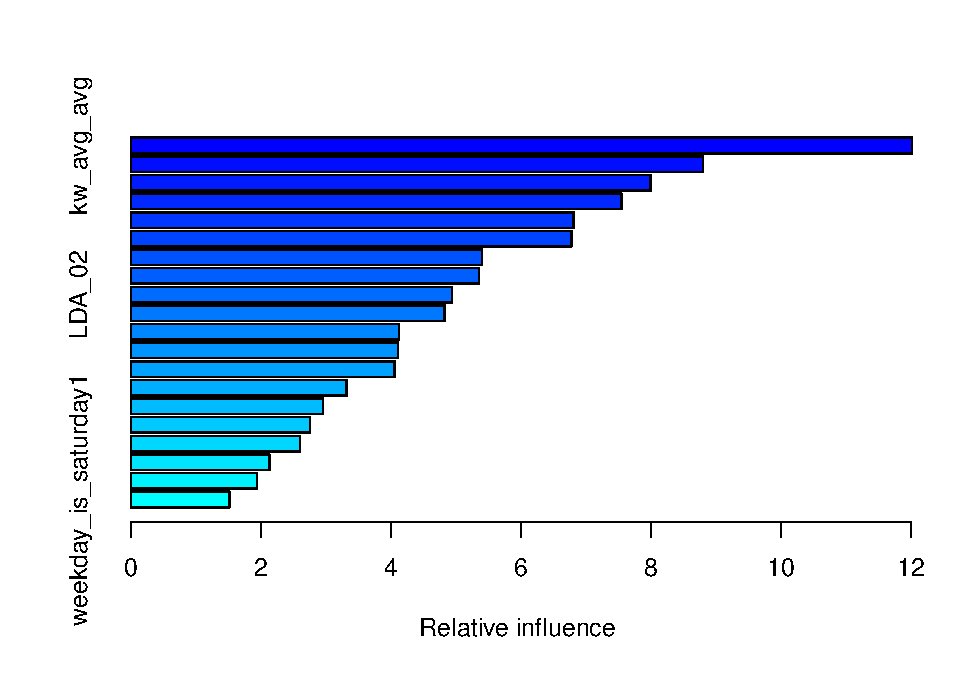
\includegraphics{news_data_prep_files/figure-latex/unnamed-chunk-6-1.pdf}

\begin{verbatim}
##                                                         var   rel.inf
## kw_avg_avg                                       kw_avg_avg 12.017824
## kw_min_avg                                       kw_min_avg  8.800135
## self_reference_min_shares         self_reference_min_shares  7.995441
## n_unique_tokens                             n_unique_tokens  7.546550
## is_weekend1                                     is_weekend1  6.809273
## kw_max_avg                                       kw_max_avg  6.776129
## kw_avg_min                                       kw_avg_min  5.403889
## kw_max_max                                       kw_max_max  5.354381
## LDA_02                                               LDA_02  4.943786
## self_reference_avg_sharess       self_reference_avg_sharess  4.827731
## data_channel_is_socmed               data_channel_is_socmed  4.125189
## data_channel_is_entertainment data_channel_is_entertainment  4.112435
## kw_avg_max                                       kw_avg_max  4.059483
## LDA_01                                               LDA_01  3.322367
## global_subjectivity                     global_subjectivity  2.954684
## LDA_03                                               LDA_03  2.755662
## title_sentiment_polarity           title_sentiment_polarity  2.602275
## data_channel_is_tech                   data_channel_is_tech  2.129581
## LDA_00                                               LDA_00  1.943311
## weekday_is_saturday1                   weekday_is_saturday1  1.519874
\end{verbatim}

\begin{Shaded}
\begin{Highlighting}[]
\NormalTok{gbm.pred <-}\StringTok{ }\KeywordTok{predict}\NormalTok{(model_gbm, news_test )}
\NormalTok{gbm.probs <-}\StringTok{ }\KeywordTok{predict}\NormalTok{(model_gbm, news_test,}\DataTypeTok{type=}\StringTok{"prob"}\NormalTok{)}
\NormalTok{gbm.confmat <-}\StringTok{ }\KeywordTok{confusionMatrix}\NormalTok{(gbm.pred, news_test}\OperatorTok{$}\NormalTok{popular, }\DataTypeTok{positive =} \StringTok{"yes"}\NormalTok{)}

\NormalTok{gbm.confmat}
\end{Highlighting}
\end{Shaded}

\begin{verbatim}
## Confusion Matrix and Statistics
## 
##           Reference
## Prediction   no  yes
##        no  1269  728
##        yes  676 1327
##                                          
##                Accuracy : 0.649          
##                  95% CI : (0.634, 0.6638)
##     No Information Rate : 0.5138         
##     P-Value [Acc > NIR] : <2e-16         
##                                          
##                   Kappa : 0.298          
##                                          
##  Mcnemar's Test P-Value : 0.1735         
##                                          
##             Sensitivity : 0.6457         
##             Specificity : 0.6524         
##          Pos Pred Value : 0.6625         
##          Neg Pred Value : 0.6355         
##              Prevalence : 0.5138         
##          Detection Rate : 0.3317         
##    Detection Prevalence : 0.5008         
##       Balanced Accuracy : 0.6491         
##                                          
##        'Positive' Class : yes            
## 
\end{verbatim}

\begin{Shaded}
\begin{Highlighting}[]
\KeywordTok{varImp}\NormalTok{(model_gbm)}
\end{Highlighting}
\end{Shaded}

\begin{verbatim}
## gbm variable importance
## 
##                               Overall
## kw_avg_avg                    100.000
## kw_min_avg                     69.349
## self_reference_min_shares      61.684
## n_unique_tokens                57.408
## is_weekend1                    50.385
## kw_max_avg                     50.069
## kw_avg_min                     36.998
## kw_max_max                     36.526
## LDA_02                         32.615
## self_reference_avg_sharess     31.510
## data_channel_is_socmed         24.817
## data_channel_is_entertainment  24.696
## kw_avg_max                     24.191
## LDA_01                         17.170
## global_subjectivity            13.668
## LDA_03                         11.772
## title_sentiment_polarity       10.311
## data_channel_is_tech            5.808
## LDA_00                          4.034
## weekday_is_saturday1            0.000
\end{verbatim}


\end{document}
